\documentclass[a4paper,11pt]{report}
\usepackage[T1]{fontenc}
\usepackage[utf8]{inputenc}
\usepackage{lmodern}
\usepackage{graphicx}
\usepackage{amsmath}
\usepackage{amssymb}
\usepackage{algpseudocode}
\title{Hardware RSA Accelerator}
\author{Group 3: Ariel Anders, Timur Balbekov, Neil Forrester}


\begin{document}

\maketitle
\tableofcontents

\begin{abstract}
%Project Objective Describe the goal of the project. What problem are you trying to solve? How is the FPGA involved in the solution of that problem? Include relevant specific details such as the target frame rate, bit rate, frame dimensions, or message sizes.
Our project is implementing the RSA cryptographic algorithm in Bluespec.
The benefits of doing this in hardware are higher performance, reduced power usage and size, and cost.
Having reusable IP that implements RSA would allow a device manufacturer to either reduce their
power footprint, or skip inclusion of a processor in a device that otherwise would not need one.  

More specifically, our objective is to implement the encryption and decryption protocols in RSA for 1024 bit messages on the Virtex5 FPGA using Bluespec.
As our implementation wouldn't be useful if the performance was too low, we tried to get throughput at least equal to that
of an implementation running in software on a Raspberry Pi (a \$35 single board computer with an ARM processor).
We also wanted the clock frequency to be above 50MHz.
After tuning the design and making appropriate trade offs, we achieved both of these goals.
\end{abstract}
%%%
\chapter{Background}
% CITE WIKIPEDIA!! - really? it doesn't seem necessary. These algorithms are quite well known, and it's clear we didn't invent them ourselves.
% 5 seconds on google will get the reader a wikipedia link anyway if they really want one.

%Assume the readers of your final report are not intimately familiar with your project domain. Provide enough high level background about the domain or algorithms involved for the reader to get an idea of the scope of the project and understand significant design choices described later in the document. Include the benefits of using an FPGA for this application.

RSA is an encryption protocol that involves a public and private key.
As indicated by its name, the public key is known to everyone and is used to encrypt messages, turning plaintext into ciphertext.
The ciphertext can then be decrypted using the private key, turning it back into plaintext.
Our implementation does not generate keys - software exists to do that already, and the benefit of doing that in hardware is low.
We perform the encryption and decryption steps, so that people can include public key cryptography in their Bluespec designs,
without employing full blown processors if they aren't otherwise necessary.
\section{RSA Algorithm}
\subsection{Definition of Variables for the RSA Algorithm}
\begin{description}
\item[Public Key ($n$, $e$)] A public key consists of the modulus $n$ and encryption exponent $e$
\item[Private Key ($n$, $d$)]A  private key consists of the same modulus $n$ and the private decryption exponent $d$
\item[Message ($m$)] The plain text message converted into an integer $m$, such that $0 \leq m \leq n$ 
\item[Ciphertext ($c$)]  The plain text message encrypted using the public key
\end{description}
\subsection{Encryption}
The ciphertext is generated by encrypting the plain text message using the public key:
\begin{equation}
  c \equiv m^e\ (mod\ n)
\end{equation}
\subsection{Decryption}
The plaintext message is generated by decrypting the ciphertext message using the private key:
\begin{equation}
  m \equiv c^d\ (mod\ n)
\end{equation}
%%%
\section{RSA Algorithm for Hardware Implementation}
A naive approach to RSA would simply raise $m$ to the power of $e$ (or $c$ to the $d$, and then compute that modulo $n$.
However, since $e$ and $d$ may be 1024 bit integers, the intermediate result would take up more memory than could be constructed
using all the mass-energy of the visible universe.
A more efficient approach, such as the Right-to-left binary algorithm, is required.
\subsection{Modular Exponentiation}
The Right-to-left binary algorithm is a good compromise between speed, memory usage, and complexity.
The goal of the algorithm is to calculate $b^e \bmod m$ for very large values of $b$, $e$, and $m$.
If the bits of $e$ are $e_1, e_2 \dots e_n$:
\begin{equation}
e = \sum_{i = 0}^{n} e_i 2^i
\end{equation}
then:
\begin{equation}
b^e = \prod_{i = 0}^{n} e_i b^{(2^i)}
\end{equation}
and since:
\begin{equation}
a * b \bmod m = (a \bmod m) * (b \bmod m) \bmod m
\end{equation}
then every intermediate result can be taken modulo $m$ to keep the size of intermediate results manageable.
Therefore, the following algorithm will compute $b^e \bmod m$ in a reasonable amount of time and memory:
\begin{algorithmic}
\State $b$, $e$, and $m$ are the inputs to the algorithm.
\State $c \gets 1$
\While{$e > 0$}
    \If{$e \bmod 2 = 1$}
		\State $c \gets c * b \bmod m$
	\EndIf
	\State $b \gets b * b \bmod m$
	\State $e \gets \lfloor e / 2 \rfloor$
\EndWhile
\State $c$ is the result of the algorithm.
\end{algorithmic}
The hardware realization of this is a circular pipeline.
However, this assumes the ability to multiply two numbers modulo a third,
the naive approach to which still requires hardware too large for the FPGA.
Fortunately, as before, there is a solution.
\subsection{Interleaved Modular Multiplication}
The Interleaved Modular Multiplication algorithm computes $xy \bmod m$.
If $N$ is the size of the numbers (in bits, for example, $N = 1024$),
and $x_i$ is the $i$th bit of $x$, then the following algorithm will perform the required steps:
\begin{algorithmic}
\State $p \gets 0$
\State $i \gets N - 1$
\While{$i \geq 0$}
	\State $p \gets p * 2$
	\If{$x_i = 1$}
		\State $p \gets p + y$
	\EndIf
	\If{$p \geq m$}
		\State $p \gets p - m$
	\EndIf
	\If{$p \geq m$}
		\State $p \gets p - m$
	\EndIf
  \State $i \gets i - 1$
\EndWhile
\State $p$ is the result of the algorithm.
\end{algorithmic}
Again, this is a circular pipeline in hardware.
However, this assumes that addition and subtraction are solved problems.
Unfortunately, a ripple-carry adder (what you get when you write {\tt a + b} in Bluespec),
produces a very long propagation delay when {\tt a} and {\tt b} are 1024 bits long.
Therefore, we had to write a carry look-ahead adder in Bluespec, and use that.
The stack of a Right-to-left binary Modular Exponentiator,
built on an Interleaved Modular Multiplier,
built on a Carry Look-ahead Adder
is capable of performing RSA on an FPGA.

\section{Implementation in C}
We have a working implementation of all our algorithms in C, that we wrote from scratch.
We verified its correctness by comparing its output to libgcrypt.  
The C implementation, of course, is unable to operate directly on 1024 bit integers, so we store them as arrays of 16 bit unsigned integers.
As a result, performing bit shifts, additions, and comparisons
takes somewhat more code than it would take to perform the corresponding operations in Bluespec.
\chapter*{High-Level Design and Test Plan} 
%Describe your system at a high level. What components are running in software, what in hardware, and how do they interact? What are the inputs and outputs to the system? How is the system used? How do you test the system? Include system diagrams.
Our RSA module has three inputs: data, exponent, and modulus;
this is because the only difference between implementing encryption versus decryption is the inputs to our RSA unit.
For example, to encrypt a plain text message the input to our RSA unit is the message, the public key and its modulus
(in this case the "data" is the plain text message and the "exponent" is the public key).
The output of this unit is the encrypted ciphertext.
Alternatively, to decrypt the cipher text, the input to our RSA unit is the ciphertext, the private key and its modulus.
In our implementation, all bit lengths are 1024 bits long and the input and output to the FPGA is implemented using the SceMi test bench.

 

To verify the functionality of the RSA module, we compared the results of the encryption and decryption blocks to the results
of a software implementation. The two private keys for encryption and
decryption modules are passed by SceMi into the hardware. A SceMi testbench
pushes a message to the encryption block, along with an enable signal, message,
and public key of the software test-bench. The module generates an encrypted message,
and the software test-bench uses its private key to decrypt and verify the 
correctness of the encrypted message.

For decryption, the process is reversed: the test-bench passes in an 
encrypted message instead of plain-text, and the decryption module uses
the private key of the software test-bench to decrypt the message. Then, the test-bench
verifies the plain-text for correctness.




%%%
\chapter*{Microarchitectural Description} 
%Describe the microarchitecture of your project. What are the component modules of your design and how do they interact? What significant design decisions led you to your microarchitecture?

Our project is divided into two important modules: {\tt ModExpt.bsv} and {\tt ModMultIlvd.bsv}.
\\
{\tt ModExpt.bsv} performs right-to-left binary modular exponentiation,
while {\tt ModMultIlvd.bsv} performs interleaved modular multiplication.
The modular exponentiator instantiates a modular multiplier.
The high level diagram in Figure \ref{fig-top} depicts the interface between
the modular multiplier and the modular exponentiator.
\begin{figure}
  \begin{centering}
    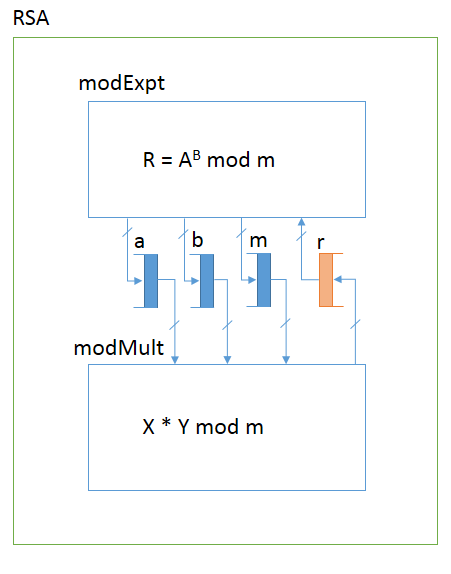
\includegraphics[scale=1]{top_level.png}
    \caption{High level overview.}
    \label{fig-top}
  \end{centering}
\end{figure}

\subsection{Right to Left Binary Modular Exponentiator}
The modular exponentiator is a circular pipeline (depicted in Figure \ref{fig-expt}).
On each cycle of the pipeline it supplies inputs to the multiplier (twice, when two operations must be performed, i.e. when the low bit of {\tt e} is non zero).
When the multiplier completes, it stores the results back into the registers.
On every iteration, the value of {\tt e} is right-shifted by one bit.
When {\tt e} is zero, the loop terminates.

\begin{figure}
  \begin{centering}
    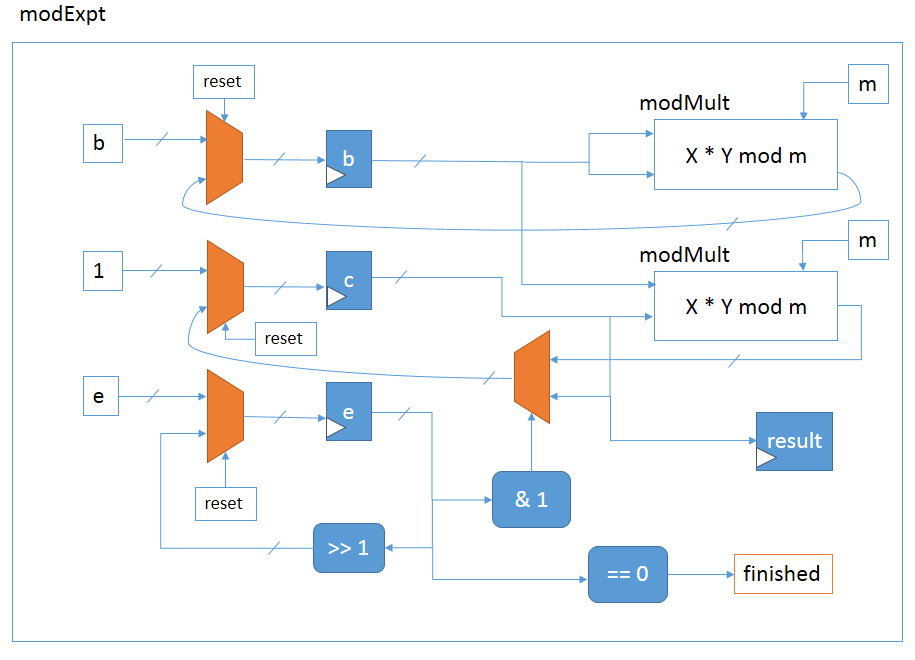
\includegraphics[width=\textwidth]{modexpt.png}
    \caption{Modular exponentiation}
    \label{fig-expt}
  \end{centering}
\end{figure}

\subsection{Interleaved Modular Multiplier}
The interleaved modular multiplier has the advantage of not requiring long multiplies, and works with
only left shifts, addition, subtraction, and comparison. Unfortunately, a step of the 
algorithm requires comparing the entire length of the data in the worst case. Additionally,
there are 3 possible add/subtract steps at every step of the algorithm. Therefore, the propagation delay
of each step of the algorithm is prohibitive without pipelining. The naive, unpipelined approach did 
meet timing because of the long propagation delay through the adders.

An overview of the module is pictured in Figure \ref{fig-inter}.

\begin{figure}
  \begin{centering}
    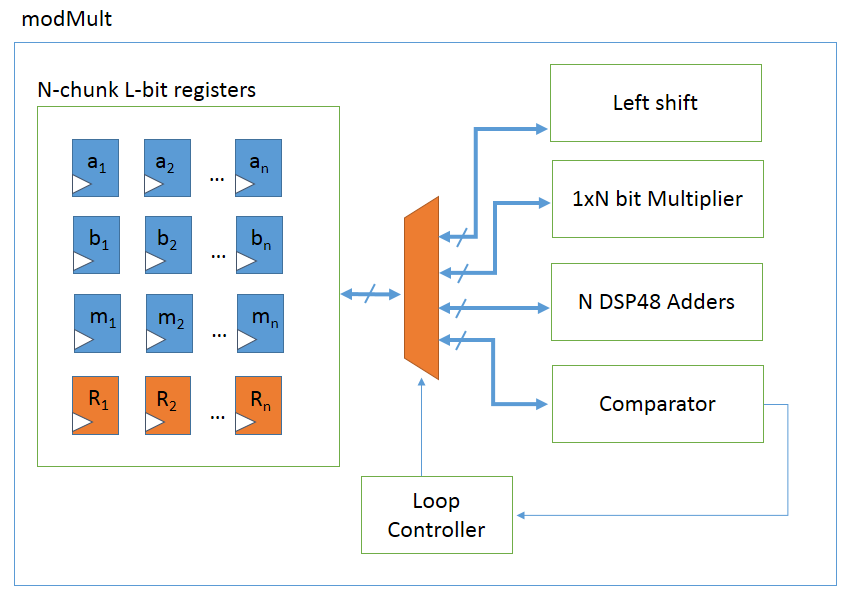
\includegraphics[width=\textwidth]{modmult.png}
    \caption{Interleaved modular multiplication}
    \label{fig-inter}
  \end{centering}
\end{figure}
\section{Implemented Modules}
The modules we implemented are:  {\tt SceMiLayer.bsv, RSAPipeline.bsv, RSA.bsv, ModMultIlvd.bsv, ModExpt.bsv, PipelineAdder.bsv, CLAdder.bsv}

\begin{description}
  \item[SceMiLayer.bsv] We developed two SceMiLayer modules to test different types of designs: one for importing vmh files, and another for importing libgcrypt for simulating our c code.  

  \item[RSAPipelinetypes.bsv] This is the general header file where we define all constant values.  This will make the overall product modular and easy for others to change core elements of design such as number of bits per chunk.
  \item[RSA.bsv]This is a dedicated alternative driver for the RSA module that performs cosimulation with libgcrypt
  \item[ModMultIlvd.bsv] The interleaved modulus multiplier based on the Montgomery Algorithm.  This function computes $a*b$ mod $m$.
  \item[ModExpt.bsv] The modulus exponentiator implements the algorithm described above.  It creates two modulus multiplier to computer $b^e$ mod $m$.
  \item[PipelineAdder, CLAdder.bsv, SlowClkAdder.bsv] These modules implement folded, carry look-ahead, and reduced clock frequency adders respectively. 
\end{description}

\subsection{Integer Representation Explorations}
\begin{enumerate}
\item The first interface was a simple {\tt Int\#(1024)} representation. We created a simple adder in order to synthesize our design.
      This is what we wound up using.
\item The second type of interface is most similar to our C implementation where integers are stored as 64 - 16 bit chunks.
\item The third type of interface uses BRAM to store chunks of the integer throughout the implementation. (This is currently incomplete)
\end{enumerate}
\subsubsection{Difficulties Encountered}
We created a simple adder in order to synthesize our design.  Since we had doubts about the success of this representation this was a vital step before continuing our design. Our concerns were well-founded for the simple {\tt Int\#(1024)} representation: the simple addition of two {\tt Int\#(1024)} were unable to synthesize.
We discuss the solutions to this and other problems later.
%%%
\chapter*{Implementation Evaluation}
 %What challenges or surprises did you face in implementing your
%design? Did you end up making changes to your original microarchitecture? Did you encounter
%any problems moving the design from simulation to the FPGA?
%Describe the results of your implementation. How many lines of Bluespec code did you have to
%write or modify? What existing IP blocks were you able to make use of in your design (DDR,
%dividers, etc...). What was the device utilization of your design, the clock frequency, and the
%high level throughput (frames per second, bits decoded per second, etc...). Did you meet your
%initial project goals? Why or why not?

\section{Challenges}
The primary challenges we encountered were making our design fit on the FPGA, and run fast enough.
We made many small tweaks to our design to meet these goals.
In order to reduce resource utilization, we scrapped most of the FIFOs in our design,
replacing them with Actions and ActionValues that directly modified the state of the modules.
Additionally, we made larger changes to the following modules:

\subsection{Modular Exponentiation}
In the modular exponentiator we traded off parallelism for lower resource utilization by instantiating one modular multiplier and making
two consecutive requests per iteration.
We originally intended to use two instances of the module to which we would make requests concurrently, but this took too much space.

\subsection{Interleaved Modular Multiplication}
\label{sec:multiple-adders}
Full length comparisons are nearly as bad a ripple carry adders in terms of propagation delay (more on adders later).
Unfortunately, the interleaved modular multiplication algorithm requires you to subtract the modulus from the intermediate result zero, one, or two times,
until the result is less than the modulus.
Determining if the result is less than the modulus requires a full length comparison.

Therefore, in order to increase the frequency at which we could run the design,
instead of performing a comparison to determine whether or not to call a particular subtractor,
we simply called all the subtractors at once, and selected the result later by looking only at the most significant bits of the results to see
which, if any, of the computations underflowed.
While it took more space on the FPGA, the increase in clock speed made up for it.

\subsection{Adder Implementation}
Synthesizing a naive 1024-bit ripple-carry adder did not meet timing due to the long carry chain.
Therefore, we came up with several alternative adder implementations:
\subsubsection{Carry Look-ahead Adder}
The carry look-ahead adder performs the 1024 bit addition in one cycle,
but the critical path is shorter than that for the ripple-carry adder.
However, this topology used more space and we had to modify the ModExpt architecture
to make it fit on the FPGA. With some additional tweaking, we got it to work.
\subsubsection{Multi-cycle Adder}
The multi-cycle adder splits the 1024 bit numbers into two 512 bit sections,
and performs the calculation in two clock cycles.
We did eventually get this working,
but performance was lower than with the carry look-ahead adder.
\subsubsection{Reduced Clock Frequency Adder}
This is a ripple-carry adder running at half the clock-frequency of the rest of the design.
While it simulated correctly, and passed synthesis,
the synchronizing FIFOs required for it to operate correctly took up nearly the entire FPGA,
and place-and-route ran for hours without finding a way to make it fit.
We could have reduced the width of the FIFOs, and passed operands through in chunks,
but performance would have been terrible.


\section{Final Design Results: Space, Timing, and Throughput}
%What was the device utilization of your design, the clock frequency, and the
%high level throughput (frames per second, bits decoded per second, etc...). Did you meet your
%initial project goals? Why or why not?

We met our goal of creating a 1024-bit RSA module that beats the performance of the 700 MHz ARM11 on the Raspberry Pi.
We can perform approximately 5 modular exponentiations per second,
while the Raspberry Pi takes several seconds to perform a single modular exponentiation.

Our design took up approximately 60\% of the FPGA:

\begin{itemize}
\item Slice registers: 42221 out of 69120  (61\%) 
\item Slice LUTs: 41574 out of 69120 (60\%)
\end{itemize}

Our design achieved a clock speed of 83.5MHz prior to place and route (which caps timing at 50MHz).



%%%

%%%
\chapter*{Design Exploration}

We have a working implementation, and it meets our performance targets.
Given more time, however, we would like to explore alternative exponentiation
and multiplication algorithms that could offer better performance.
Furthermore, our entire device performs one operation at a time.
During the vast majority of this time the execution of the modular exponentiation
module is blocked, waiting for the modular multiplication module to finish a computation.
If we had a larger FPGA to work with, we could instantiate multiple
modular multiplication modules, and have a single modular exponentiator hand out jobs to them.
That way it could perform many operations at once, and increase the performance to size ratio.

We would also like to implement probabilistic multi-cycle comparisons to get around the multiple-subtractor trick we described in Section \ref{sec:multiple-adders}.
The reason we had to instantiate multiple subtractors was because full-length comparisons produce a large propagation delay.
However, in almost every case it is possible to decide which of two numbers is bigger by looking only at the first few bits.
Therefore, we want to change our design so that the modular multiplier only looks at the first few bits of a number.
If it is different, then it calls the appropriate subtractor.
If the first few bits are the same, then it waits until the next clock cycle, compares the next few bits, and so on until a difference is found.
In the vast majority of cases, this will complete in one clock cycle, that clock cycle will not be excessivly long,
and it won't take up much space with extraneous subtractors.
However, when necessary, this will take several clock cycles to complete.
The only reason we haven't made this change already is that we ran out of time, and our design works as it is.

We also have various ideas about how we might use BRAM to improve our design.
However, we never got around to fully exploring any of these.
Given more time, we would like to consider if our design could be made smaller or faster through the judicious use of BRAM modules.

\end{document}
